\documentclass[14pt]{report}
\usepackage[utf8]{inputenc}
\usepackage[russian]{babel}

\usepackage{indentfirst}
\usepackage{amsmath}
\usepackage{graphicx}
\usepackage{listings}
\usepackage{biblatex}
\usepackage{float}
\usepackage{floatrow}
\usepackage{caption}
\usepackage{enumitem}

\addbibresource{report.bib}

\usepackage{etoolbox}
\makeatletter
\patchcmd{\chapter}{\if@openright\cleardoublepage\else\clearpage\fi}{}{}{}
\makeatother

\lstset{extendedchars=\true, frame=single, numbers=left,captionpos=t}

\usepackage[left=2cm,right=2cm, top=2cm,bottom=2cm,bindingoffset=0cm]{geometry}
\usepackage{titlesec, blindtext, color}
\newcommand{\hsp}{\hspace{20pt}}
\titleformat{\chapter}[hang]{\Huge\bfseries}{\thechapter\hsp{|}\hsp}{0pt}{\Huge\bfseries}

\begin{document}
\def\chaptername{}
\thispagestyle{empty}
\begin{titlepage}
	\noindent \begin{minipage}{0.15\textwidth}
	
\includegraphics[width=\linewidth]{img/bmstu.jpg}
	\end{minipage}
	\noindent\begin{minipage}{0.9\textwidth}\centering
		\textbf{Министерство науки и высшего образования Российской Федерации}\\
		\textbf{Федеральное государственное бюджетное образовательное учреждение высшего образования}\\
		\textbf{~~~«Московский государственный технический университет имени Н.Э.~Баумана}\\
		\textbf{(национальный исследовательский университет)»}\\
		\textbf{(МГТУ им. Н.Э.~Баумана)}
	\end{minipage}
	
	\noindent\rule{18cm}{3pt}
	\newline\newline
	\noindent ФАКУЛЬТЕТ $\underline{\text{«Информатика и системы управления»}}$ \newline\newline
	\noindent КАФЕДРА $\underline{\text{«Программное обеспечение ЭВМ и информационные технологии»}}$\newline\newline\newline\newline\newline
	
	
	\begin{center}
		\noindent\begin{minipage}{1.3\textwidth}\centering
			\Large\textbf{  Отчет по лабораторной работe №16}\newline
			\textbf{по дисциплине "Функциональное и логическое}\newline
			\textbf{программирование"}\newline\newline
		\end{minipage}
	\end{center}
	
	\noindent\textbf{Тема} $\underline{\text{~~~~Рекурсия на Prolog~~~~~~~~~~~~~~~~~~~~~~~~~~~~~~}}$\newline\newline
	\noindent\textbf{Студент} $\underline{\text{~Варламова Е.А.~~~~~~~~~~~~~~~~~~~~~~~~~~~~~~~~~~~~}}$\newline\newline
	\noindent\textbf{Группа} $\underline{\text{~~~ИУ7-61Б~~~~~~~~~~~~~~~~~~~~~~~~~~~~~~~~~~~~~~~~~~}}$\newline\newline
	\noindent\textbf{Оценка (баллы)} $\underline{\text{~~~~~~~~~~~~~~~~~~~~~~~~~~~~~~~~~~~~~~~~~~~}}$\newline\newline
	\noindent\textbf{Преподаватель} $\underline{\text{~~~Толпинская Н.Б. Строганов Ю.В.~~~~~~~~~~~~~~~~~~}}$\newline\newline\newline
	
	\begin{center}
		\vfill
		Москва~---~\the\year
		~г.
	\end{center}
\end{titlepage}

\newpage

\section*{Задание}

Используя хвостовую рекурсию, разработать программу, позволяющую найти
\begin{enumerate}
    \item n!,
    \item n-е число Фибоначчи.
\end{enumerate}

Убедиться в правильности результатов.

Для одного из вариантов ВОПРОСА и каждого задания составить таблицу,
отражающую конкретный порядок работы системы:

Т.к. резольвента хранится в виде стека, то состояние резольвенты требуется отображать
в столбик: вершина – сверху! Новый шаг надо начинать с нового состояния резольвенты!

\section*{Код программы}

\vspace{\baselineskip}

\begin{lstlisting}[language=Prolog]
domains
  num = integer

predicates
  fact(num, num)
  rec_fact(num, num, num)

  fib(num, num)
  rec_fib(num, num, num, num)

clauses
  rec_fact(N, Res, Acc) :- N > 1, 
                          NewN = N - 1, 
                          NewAcc = Acc * N, 
                          rec_fact(NewN, Res, NewAcc), !.
  rec_fact(_, Res, Acc) :- Res = Acc.
  fact(N, Res) :- rec_fact(N, Res, 1), !.

  rec_fib(N, F1, F2, Res) :- N > 2, 
                             NewF1 = F2, 
                             NewF2 = F1 + F2, 
                             NewN = N - 1, 
                             rec_fib(NewN, NewF1, NewF2, Res), !.
  rec_fib(_, _, B, Res) :- Res = B.
  fib(N, Res) :- rec_fib(N, 1, 1, Res).

goal
  %fact(5, Res).
  %fib(7, Res).
\end{lstlisting}

\vspace{\baselineskip}

\newpage

\textbf{Вопрос №1}\\

\begin{figure}[H]
	\centering
	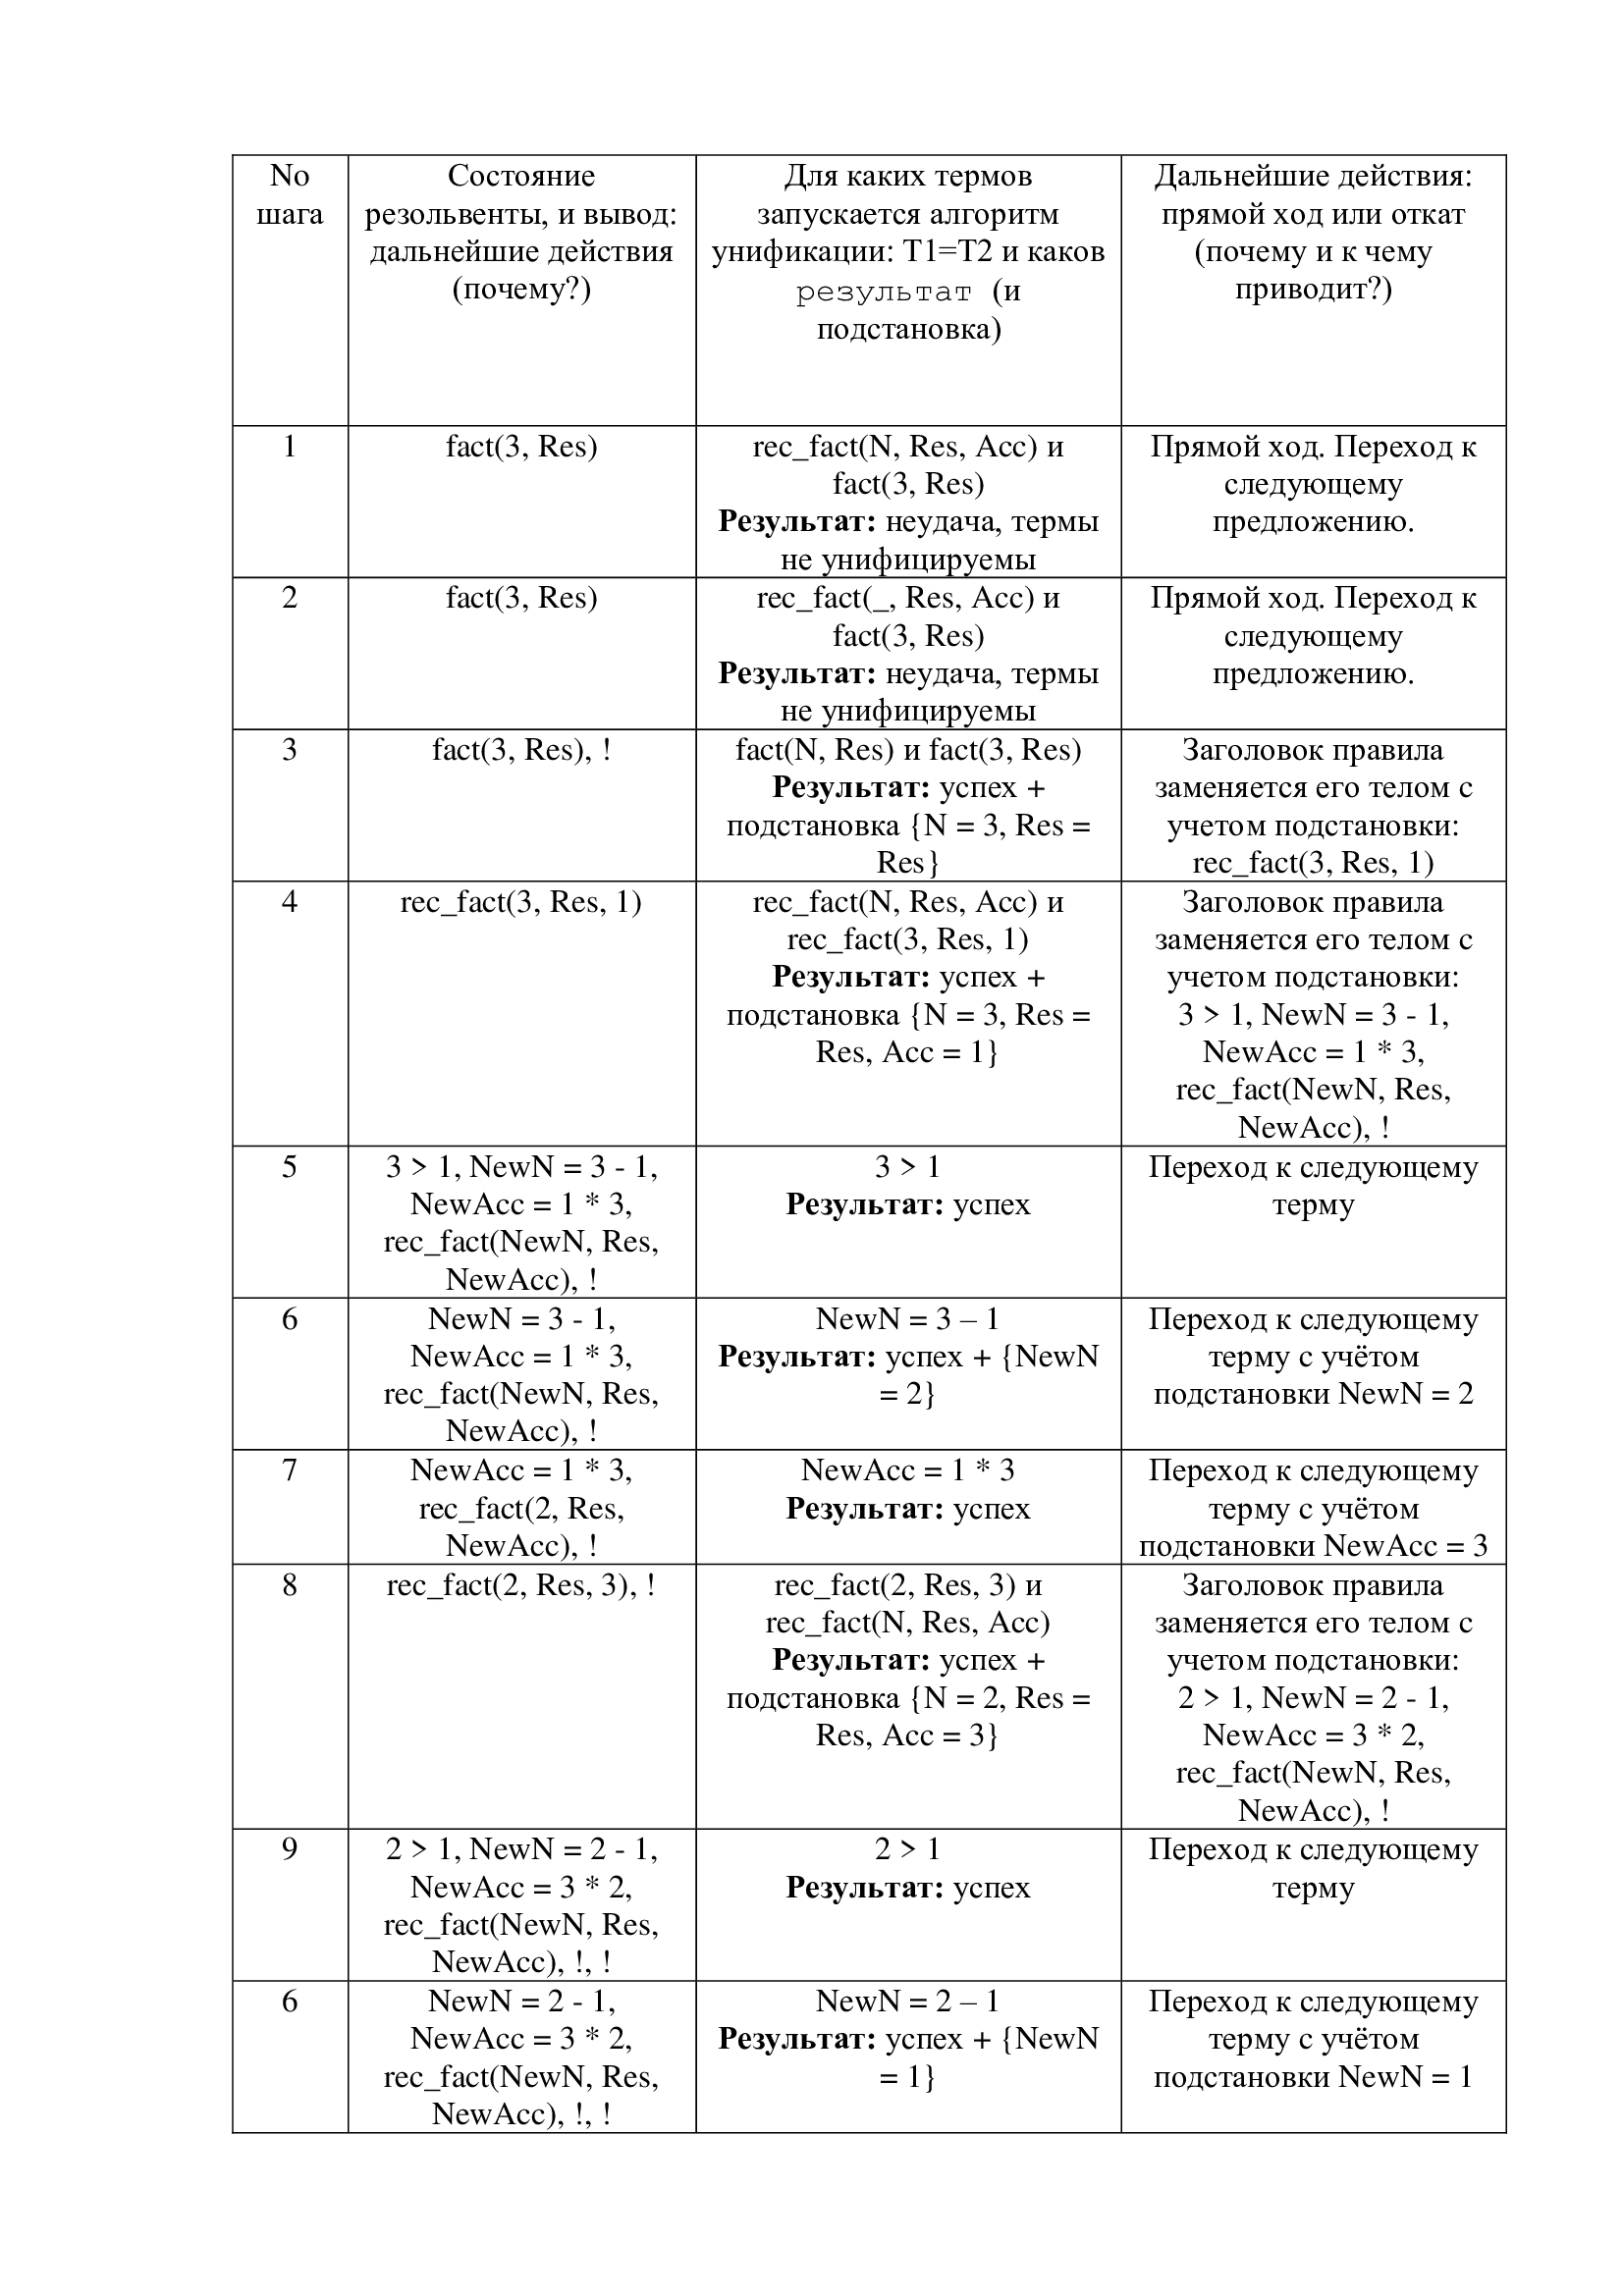
\includegraphics[scale=0.26]{0.jpg}
	\caption{Таблица к вопросу № 1.}
	\label{d:matr_rec}
\end{figure}

\begin{figure}[H]
	\centering
	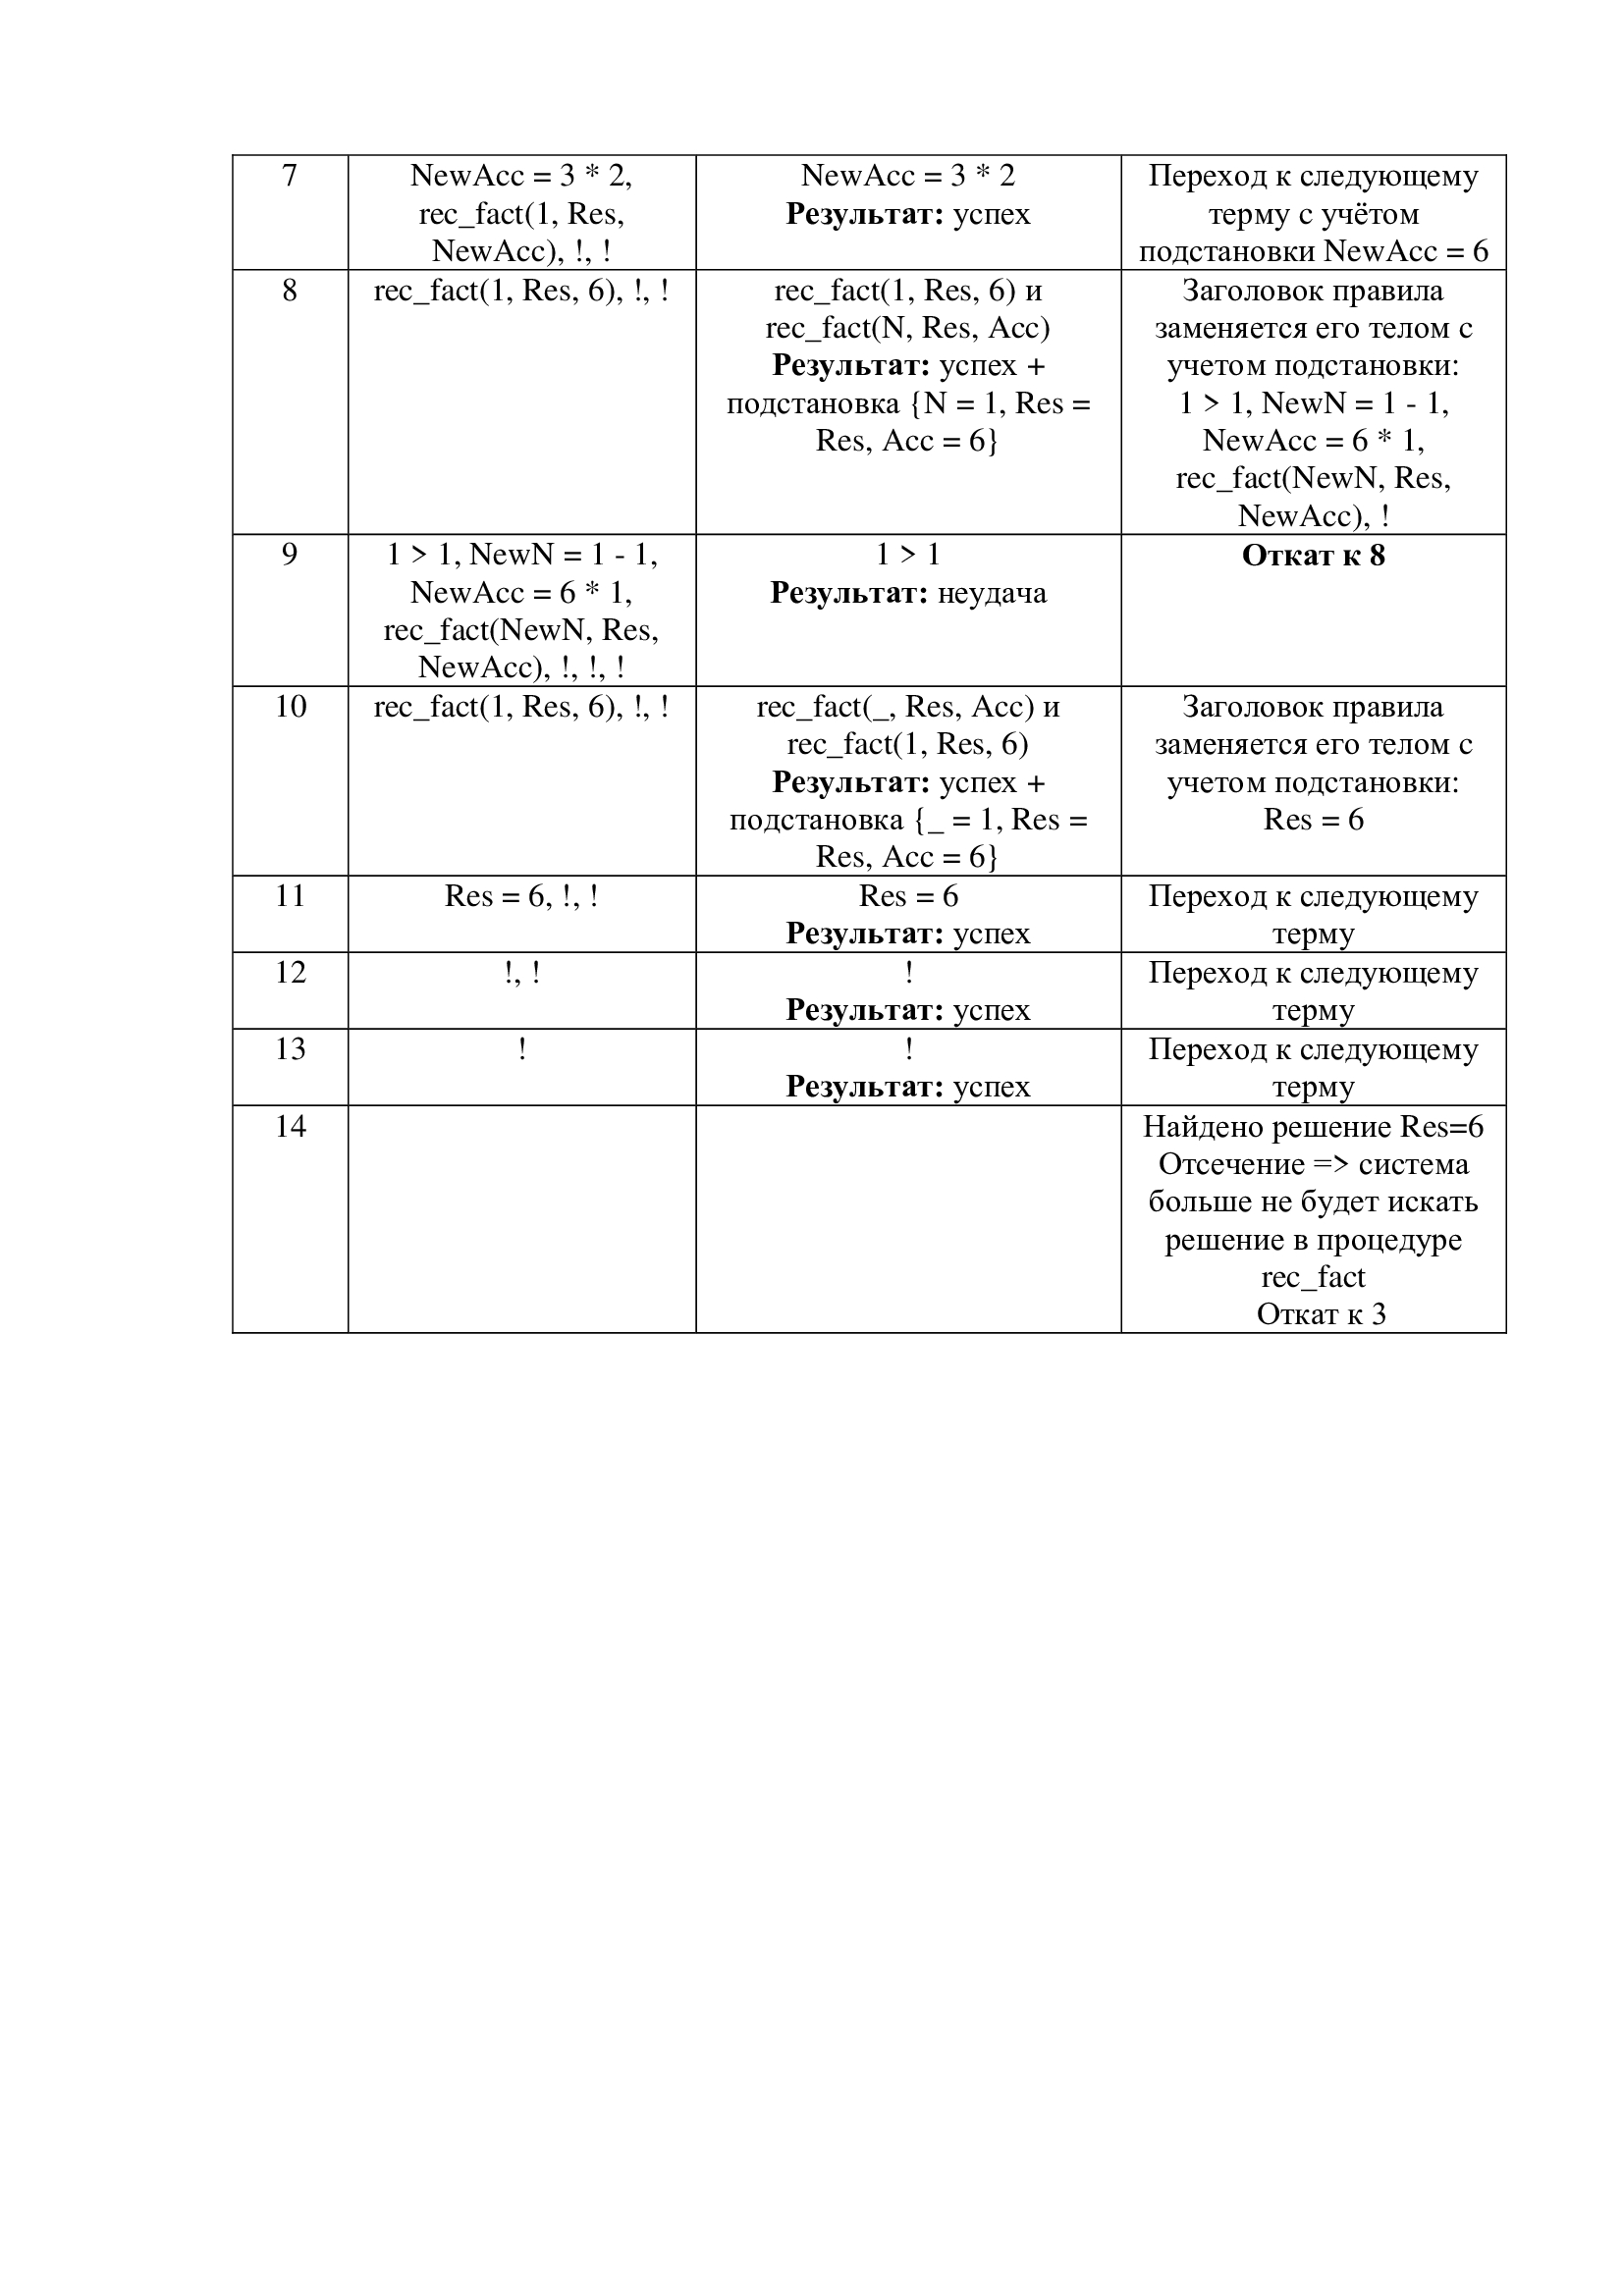
\includegraphics[scale=0.26]{1.jpg}
	\caption{Таблица к вопросу № 1.}
	\label{d:matr_rec}
\end{figure}

\end{document}
